%********************************************************************
% Define document class
%********************************************************************
\RequirePackage{fix-cm} 
\documentclass[fontsize=10pt,paper=a4,
			   oneside, %twoside for printing double-sided
			   openright,titlepage,fleqn,%
               headinclude,footinclude=true,BCOR=5mm,%
               numbers=noenddot,cleardoublepage=empty,%
               captions=tableheading,%
               %ngerman,
               british,%
               ]{scrreprt}


               
%********************************************************************
% Note: Make all your adjustments in here
%********************************************************************
\input{thesis-settings_steppchr}


%********************************************************************
% Bibliographies
%*******************************************************
\addbibresource{Literature/E49_SAPEX-DLB.bib}
\addbibresource[label=ownpubs]{Literature/steppchr_Publications.bib}

\AtEveryBibitem{\ifentrytype{article}{\clearfield{issn}}{}}

\renewbibmacro{in:}{%
	\ifentrytype{article}{}{\printtext{\bibstring{in}\intitlepunct}}}

\renewbibmacro*{volume+number+eid}{%
	\printfield{volume}%
	%  \setunit*{\adddot}% DELETED
	\setunit*{\addnbthinspace}
	\printfield{number}%
	\setunit{\addcomma\space}%
	\printfield{eid}}

\renewrobustcmd*{\bibinitdelim}{\,}

\DeclareFieldFormat[article, inbook, incollection, thesis, inproceedings]{title}{#1}
\DeclareFieldFormat[article]{volume}{\textbf{#1}}
\DeclareFieldFormat[article]{number}{\mkbibparens{#1}\addcolon}
\DeclareFieldFormat{pages}{#1}
\DeclareNameAlias{sortname}{last-first}
\DeclareNameAlias{default}{last-first}

%********************************************************************
% Hyphenation
%*******************************************************
\hyphenation{pho-to-gram-me-try boot-strap Fern-er-kund World-View for-ests dom-i-nat-ed spruce-dom-i-nat-ed 
Pretzsch Eu-ro-pean Dor-drecht to-pog-ra-phy ap-proach con-cept large-ly re-mote-ly vol-umes
al-ter-nate three-di-men-sion-al char-ac-ter-i-za-tion se-mi-em-pir-i-cal
Schwei-zer-bart Fac-tor Pub-lish-er con-cept Kli-ma-an-pas-sung Holz-wirt-schaft-liche
	}

%********************************************************************
% Acronyms
%*******************************************************
%
%\DeclareAcronym{ABA}{short = ABA , long = area-based approach}
%\DeclareAcronym{ALS}{short = ALS, long = airborne laser scanning}
%\DeclareAcronym{ACS}{short = ACS, long = angle-count sampling}
%\DeclareAcronym{BaySF}{short = BaySF, long = Bayerische Staatsforsten}
%\DeclareAcronym{CHM}{short = CHM, long = canopy height model}
%\DeclareAcronym{DAP}{short = DAP, long = digital aerial photogrammetry}
%\DeclareAcronym{DSM}{short = DSM, long = digital surface model}
%\DeclareAcronym{DTM}{short = DTM, long = digital terrain model}
%\DeclareAcronym{LiDAR}{short = LiDAR, long = Light detection and ranging}
%\DeclareAcronym{ME}{short = ME, long = mean error}
%\DeclareAcronym{NFI}{short = NFI, long = national forest inventory}
%\DeclareAcronym{NVI}{short = NVI, long = Northern Vancouver Island}
%\DeclareAcronym{oob}{short = oob, long = out-of-bag}
%\DeclareAcronym{PAI}{short = PAI, long = periodic annual increment}
%\DeclareAcronym{RF}{short = RF, long = random forest}
%\DeclareAcronym{RMSE}{short = RMSE, long = root mean squared error}
%\DeclareAcronym{SGM}{short = SGM, long = semi-global matching}
%\DeclareAcronym{WV2}{short = WV2, long = WorldView-2}

%\sloppy % für besseren Blocksatz


% include only those files for actual compilation
\includeonly{
	FrontBackMatter/TUMtitle,
	FrontBackMatter/Titlepage,
	FrontBackMatter/Titleback,
	FrontBackMatter/Dedication,
	FrontBackMatter/Abstract,
	FrontBackMatter/Publications,
	FrontBackMatter/Acknowledgements,
	Chapters/01_Introduction,
	Chapters/02_Materials,
	Chapters/03_Methods,
	Chapters/04_Results,
	Chapters/05_Discussion,
	Chapters/06_Conclusion,
	%Chapters/AA_Appendix,
	FrontBackMatter/Bibliography,
	FrontBackMatter/Index}


% ********************************************************************
% Start of Document
%*******************************************************
\begin{document}
\frenchspacing
\selectlanguage{british}
\pagenumbering{roman}
\pagestyle{plain}





%******************************************************************
% Frontmatter
%******************************************************************
\begin{titlepage}


\sffamily

\begin{addmargin}[-1.5cm]{-1.5cm}

\begin{center}


\includegraphics[height=18mm]{Figures/TUM_Logos/tumlogo}

%%% for including both the TUM and the WZW logo in one line
%\includegraphics[height=18mm]{Figures/TUM_Logos/WZW} \hfill
%\includegraphics[height=18mm]{Figures/TUM_Logos/tumlogo}


\bigskip

\LARGE{\spacedlowsmallcaps{\myUni}}

\medskip

\large{\myDepartment}

\bigskip
\bigskip
\bigskip

{\LARGE\spacedlowsmallcaps{\textcolor{tumblau}{\myTitle}} \\
}

\bigskip
\bigskip

{\Large\spacedlowsmallcaps{\myName}} \\

\bigskip
\bigskip
\bigskip

\end{center}

\noindent\large{Complete copy of the dissertation approved by the \myFaculty of the \myUni in partial fulfillment of the requirements for the degree of} 

\medskip

\centerline{\emph{\myDegree}}

\bigskip
\bigskip
\medskip


%\noindent{Chair:}
%
%\begin{description}
%	\item[] Univ.-Prof. Dr.-Ing. Stephan Pauleit
%\end{description}			 	
%
%\medskip
%
%\noindent{Dissertation examiners:} 
%
%	\begin{enumerate}
%	\item Univ.-Prof. Dr. Dr. h.c. Hans Pretzsch
%	\item Univ.-Prof. Dr. Thomas Knoke
%	\item Univ.-Prof. Dr. Clement Atzberger\\ (Universität für Bodenkultur Wien)
%\end{enumerate}



\begin{center} 
%  \vspace{2mm}
   \begin{tabular}{llll}
	Chair: 				   & &    & Univ.-Prof. Dr.-Ing. Stephan Pauleit\\[4mm]                                            
    Dissertation examiners:& & 1. & Univ.-Prof. Dr. Dr. h.c. Hans Pretzsch\\[2mm]
                           & & 2. & Univ.-Prof. Dr. Thomas Knoke\\[2mm]
                           & & 3. & Univ.-Prof. Dr. Clement Atzberger \\
                           & &    & (Universität für Bodenkultur Wien) \\
  \end{tabular}
\end{center}


							
							
\bigskip
\bigskip
\bigskip

\noindent\large{The dissertation was submitted to the \myUni on \today{} and accepted by the TUM School of Life Sciences Weihenstephan on \underline{\phantom{\DTMdisplaydate{2016}{05}{30}{-1}}}	.}


\end{addmargin}



\end{titlepage}

  %den muss ich am Schluss nochmal anpassen
%*******************************************************
% Titlepage
%*******************************************************

\begin{titlepage}
\pdfbookmark{Titlepage}{Titlepage}
\begin{addmargin}[-1cm]{-1cm}

	\null\vfill
	
	\begin{center}
		\large
		
		{\spacedlowsmallcaps{\myName}} \\
	
		\bigskip
		\bigskip
	
		{\Large\spacedlowsmallcaps{\textcolor{tumblau}{\myTitle}} \\
		}
		
		
	
		\bigskip
		    
		\vspace{14cm}
		
		\begin{tabular} {cc}
		\parbox{0.3\textwidth}{\includegraphics[width=2.5cm]{Figures/Picto_Airplane_Trees/Picto_Airplane_Trees}}
		&
		\parbox{0.7\textwidth}{{\Large\spacedlowsmallcaps{\mySubTitle}} \\ 
		
							{\normalsize
							
							\myFaculty \\
							\myUni \\
							
							\medskip
							\myLocation \\
							\myTime}}
					\end{tabular}
	\end{center}
	\vfill
\end{addmargin}
\end{titlepage}




%*******************************************************
% Titleback
%*******************************************************
\thispagestyle{empty}

\hfill

\vfill

\noindent\myName:
\textit{\myTitle,} \\
\mySubTitle, \textcopyright\ \myTime.

%\medskip
%\noindent{\spacedlowsmallcaps{Website}}: \\
%\url{htt:/www.lwf.bayern.de/}
%\myUrl

\medskip
\noindent{\spacedlowsmallcaps{E-mail}}: \\
\mail{c.stepper@mytum.de}

\medskip
\noindent{\spacedlowsmallcaps{Supervisor}}: \\
Prof. Dr. Dr. h.c. Hans Pretzsch

\vspace{1cm}
\hrule
\bigskip

\noindent The title page shows an artwork displaying the acquisition of overlapping digital aerial images and trees measured on ground plot (own drawing).

\noindent This document was set in \LaTex{}.


\cleardoublepage%*******************************************************
% Dedication
%*******************************************************
\thispagestyle{empty}
%\phantomsection 
\refstepcounter{dummy}
\pdfbookmark[1]{Dedication}{Dedication}

\vspace*{3cm}

\begin{center}

%    You don't choose your family. \\
%    They are God's gift to you, as you are to them. \\ \medskip
%    --- Desmond Tutu 
%    
%    \bigskip
%    
    I have found the best way to give advice to your children \\
     is to find out what they want and then advise them to do it. \\ \smallskip
     \emph{--- Harry S. Truman}

      
\end{center}

\bigskip
\bigskip

\begin{center}
    Dedicated to the loving parents Elisabeth and Ludwig Stepper. 
\end{center}
\cleardoublepage%*******************************************************
% Abstract + Zusammenfassung
%*******************************************************

\pdfbookmark[1]{Abstract}{Abstract}
\begingroup
\let\clearpage\relax
\let\cleardoublepage\relax
\let\cleardoublepage\relax

\chapter*{Abstract}
Information about canopy height and spatial structure is essential for various tasks in forest planning and management. Retrieving this information from remote sensing data has been focus in research as this technique opens the possibility to assess large forested areas. 
The work presented in this thesis focussed on utilizing digital aerial imagery from airborne platforms to generate accurate measurements of canopy height by means of image matching algorithms. Together with ground information, necessary for model calibration, different forest inventory attributes can be assessed \dots

\vfill

\begin{otherlanguage}{ngerman}
	\pdfbookmark[1]{Zusammenfassung}{Zusammenfassung}
	
\chapter*{Zusammenfassung}
Informationen über die Bestandeshöhe und die räumliche Verteilung der Bäume in einem Bestand \dots 

\end{otherlanguage}



\endgroup			

\vfill


\cleardoublepage%*******************************************************
% Publications
%*******************************************************
\pdfbookmark[1]{Publications}{publications}
\chapter*{Publications}\graffito{List of scientific papers included in this thesis}
This dissertation was done in a publication-based manner. The developed methods, results, and findings were published in different scientific papers: 

%\noindent Put your publications from the thesis here. The packages \texttt{multibib} or \texttt{bibtopic} etc. can be used to handle multiple different bibliographies in your document.

\begin{refsection}[ownpubs]
    \small
    \nocite{*} % is local to the enclosing refsection
    \printbibliography[heading=none]
\end{refsection}

%\emph{Attention}: This requires a separate run of \texttt{bibtex} for your \texttt{refsection}, \eg, \texttt{ClassicThesis1-blx} for this file. You might also use \texttt{biber} as the backend for \texttt{biblatex}. See also \url{http://tex.stackexchange.com/questions/128196/problem-with-refsection}.
\cleardoublepage%*******************************************************
% Acknowledgements
%*******************************************************
\pdfbookmark[1]{Acknowledgements}{Acknowledgements}

\begin{flushright}{\slshape    
		In general, the remote sensing problem \\
		can be presented as inferring the order \\ 
		in the properties and distributions of matter \\ 
		and energy in the scene from the set \\
		of measurements comprising the image.} \\ \medskip
%		--- \defcitealias{Strahler:1986}{Alan H. Strahler et al. 1986}\citetalias{Strahler:1986} \citep{Strahler.1986}
		--- \cite{Strahler.1986}
		
	
\end{flushright}


\begingroup
\let\clearpage\relax
\let\cleardoublepage\relax
\let\cleardoublepage\relax

\chapter*{Acknowledgements}

I would like to take the opportunity to thank all those involved in the work I did in the last years.
Without your help and support, I would not have been able to mastering the challenges on my way to this thesis.

First of all, I express my gratitude to Prof.\,Dr.\,Hans Pretzsch, 
who complied to supervise me as external Ph.D. Student at Technische Universität München. 
He always encouraged me to pursue on my objectives and supported me with his great experience in scientific work.
His different perspective to my work, underpinned by his enormous knowledge in forest growth and yield, added great value to my research; 
our meetings often resulted in very fruitful discussions developing new ideas and hypotheses.

I am thankful to Prof.\,Dr.\,Thomas Knoke for his willingness to act as second examiner
and to Prof.\,Dr.\,Stephan Pauleit for taking over the chair of the committee.
Many thanks go to Prof.\,Dr.\,Clement Atzberger from the University of Natural Resources and Life Sciences 
for agreeing to examine this thesis, but much more for many helpful discussions and advises.  

I am very thankful to Dr.\,Christoph Straub. 
You have been a great colleague, a perfect partner and an ongoing supporter.
I enjoyed it very much collaborating with you. 
Many thanks also go to Rudolf Seitz for giving me the opportunity to work in this project, 
to Helena Löffler, Kristine Meyerhofer, and Oliver Bauer for sharing their ideas, skills and coffee breaks,
and all my colleagues at the \myInstitute. 
A special thanks goes to Michael Suda for running together criss-cross around Freising.
Not only the sports, but also our conversations did me good.   
 
I am very grateful to Markus Immitzer for his invaluable aid during working on different aspects of this thesis. 
Thanks for sharing your knowledge in the \textsf{R} programming language, 
for very in-depth discussions and constructive feedback, 
and for the possibility to co-author a terrific paper.    

I owe special thanks to Joanne White, Mike Wulder (Canadian Forest Service),
Nicholas Coops, Piotr Tompalski (Integrated Remote Sensing Studio, UBC) and the complete crowd of IRSS for giving me the chance to work abroad in a very inspiring team. 
You made one of the best experiences during my Ph.D. possible. 
I am also very thankful to Brynn McMillan for sharing a great time in Vancouver. 

\noindent Finally, many thanks to \emph{Melanie}. You always believed in me. I'm so happy that you're with me.

\endgroup




\pagestyle{scrheadings} 
\cleardoublepage\input{FrontBackMatter/Contents}


%******************************************************************
% Mainmatter
%******************************************************************

\cleardoublepage
\pagenumbering{arabic}

  \begin{linenumbers}

%\part{Preliminary notes}
%
%\chapter*{TUM PhD regulations}
%
%\begin{otherlanguage}{ngerman}
%\begin{itemize}
%	\item Bei einer publikationsbasierten Dissertation sind in knapper Fassung das wissenschaftliche Problem, die verwendeten Lösungsansätze, die erzielten Ergebnisse und Schlussfolgerungen sowie die in Bezug stehende Literatur darzustellen. 
%	\item Die Dissertation muss selbständig angefertigt sein. Sie muss eine Zusammenfassung des Inhalts und ein vollständiges Verzeichnis der benutzten Literatur sowie weiterer Informationsquellen enthalten.
%	\item Kriterien für die publikationsbasiserte Promotion
%	\begin{itemize}
%		\item Einleitungs- und Methodenteil (20 Seiten). Ein themenübergreifender Diskussionsteil mit Reflexion zur bestehenden Literatur. 
%		\item Kumulative Einbindung von mindestens zwei akzeptierten Erstautorenveröffentlichungen (full paper in einem englischsprachigen, international verbreiteten Publikationsorgan, peer reviewed) 
%		\item Die eingebundenen Veröffentlichungen müssen federführend vom Doktoranden abgefasst sein. 
%		\item Eingebunden muss sein: je eine einseitige Zusammenfassung der jeweiligen Veröffentlichungen unter Hervorhebung der individuellen Leistungsbeiträge des Kandidaten. 
%	\end{itemize}
%\end{itemize}
%\end{otherlanguage}


\part[Digital Aerial Photogrammetry in Forestry]{\myTitle}

%************************************************
\chapter{Introduction}
\label{chp:Introduction}
%************************************************

Digital aerial photogrammetry experienced increased attention during the last decade. 


\section{State of the Art}\label{sec:State}

Literature review on remote sensing applications in forestry. Historic development of aerial imagery for use in forest inventory and management planning.

Early developments of aerial photogrammetry for height retrieval - theoretical framework

3d remote sensing technologies: Airborne laser scanning as method of choice.

Here we want to cite \cite{Stepper.2015b}




\section{Research Objectives}\label{sec:Objectives}

The research presented in this thesis focussed on the following objectives:

\begin{enumerate}
	
	\item Are digital aerial images acquired within the standardized administrative aerial surveys suitable to computed dense image-based point clouds or digital surface models, that characterize the forests' surface with a sufficient level of detail?
	
	\item Can Semi-global matching point clouds, normalized to heights above ground using ALS-based DTMs, be used to model key forest inventory attributes, e.g. gross volume?
	
	\item Are repeated aerial image acquisitions and the derived CHMs capable to assess canopy height changes is a complex temperate forest?
	
\end{enumerate}






%************************************************
\chapter{Materials}
\label{chp:Mat}
%************************************************


\section{Study Areas}\label{sec:StudyAreas}\index{study area}

The research studies, which are compiled in the present work, were conducted using remote sensing data and ground based measurements
from different test sites\index{test site|see{study area}} 
(see Figures~\ref{fig:TestSites_BY} and \ref{fig:TestSite_NVI}, and Table~\ref{tab:TestSites}).
The selection \graffito{Selection criteria for the study areas in \emph{Bavaria}.} of the test sites in \emph{Bavaria}, 
Germany, was made in order to best meet the following criteria:

\begin{itemize}
	\item Field inventory measurements of recent date are available for larger contiguous forested areas.
	\item Lapse of time between the acquisition of the airphotos and the ground based measurements is as short as possible.
	\item Test sites represent different forest conditions, including topography, climate, tree species, tree species mixture, 
		and forest management practice.
\end{itemize}

\noindent The test site on \emph{\ac{NVI}} was selected \graffito{A comparative analysis of \ac{ALS}- and \ac{DAP}-based height data
	was possible for the \ac{NVI} test site.}
in order to scrutinize the developed methods 
under largely different conditions, \ie, among other factors, the areal extent of the test site, the prevailing tree species, the applied forest management, 
and the different strategy for ground data acquisition. Timely coincident data of \ac{ALS} and aerial photography were available for the \ac{NVI} area,
which allowed for a comparative analysis of both remote sensing data types for use in forest inventory applications.   

\begin{threeparttable}[t]
	\myfloatalign
	\caption[Overview of test sites.]{Overview of the different test sites in Bavaria, Germany, and British Columbia, Canada.}
	\label{tab:TestSites}
	\small
	\begin{tabularx}{\textwidth}{p{2.7cm}p{.7cm}p{2.6cm}X}
		\toprule
		\tableheadline{Test site} & \spacedlowsmallcaps{Area} \linebreak \footnotesize{[km\textsuperscript{2}]} & \spacedlowsmallcaps{dominant tree species} &  \tableheadline{Studies}  \\ 
		\midrule
		\emph{Spessart}\linebreak(northwestern \newline Bavaria) & 446 & European beech, sessile oak & \cite{Straub.2016}  \\ 
		\emph{Steigerwald} \linebreak (northwestern \newline Bavaria)&  556 &  European beech, sessile oak & \cite{Stepper.2015b};\newline \cite{Immitzer.2016}; \newline \cite{Stepper.2016} \\
		\emph{Frankenwald} \linebreak (northeastern \newline Bavaria) & 396 &  Norway spruce &\cite{Straub.2016};\newline \cite{Stepper.2016}  \\ 
		\emph{Traunstein} \linebreak (southeastern \newline Bavaria) & 90 & Norway spruce, European beech, white fir & \cite{Stepper.2015}  \\ 
		\emph{Northern \linebreak Vancouver Island} \linebreak(British Columbia) & 662 & Western hemlock, Western red cedar &  \cite{White.2015}  \\ 
		\bottomrule
	\end{tabularx}
	\begin{tablenotes}
			\item \footnotesize{\textbf{Note:} detailed descriptions of the test sites are given in the respective research papers. Deviating figures for area sizes are due to use of different subsets for the studies.}
	\end{tablenotes}	
\end{threeparttable}
	

%\begin{sidewaystable}[h]
%\begin{threeparttable}
%	\myfloatalign
%	\caption[Overview of test sites.]{Overview of the different test sites in Bavaria, Germany, and British Columbia, Canada.}
%	\label{tab:TestSites}
%	\begin{tabularx}{\textwidth}{llrXrXl} \toprule
%		\tableheadline{Test site} & \tableheadline{Location} & \tableheadline{Area \textnormal{[\,km\textsuperscript{2}]}} & \tableheadline{Tree Species} & \tableheadline{\textnumero \: processed airphotos} & \tableheadline{\textnumero \: ground sampling plots} & \tableheadline{Studies}  \\ 
%		\midrule
%		\emph{Steigerwald} & Northwestern Bavaria & 413 &  European beech, sessile oak&  & 3937 &\cites{Stepper.2015}{Immitzer.2016}{Stepper.2016}\\
%		\emph{Spessart} & Northwestern Bavaria & 228 & European beech, sessile oak &  & 2010 & \cite{Straub.2016}  \\ 
%		\emph{Frankenwald} & Northeastern Bavaria & 231 &  Norway spruce &  & 2267 &\cites{Straub.2016}{Stepper.2016}  \\ 
%		\emph{Traunstein} & Southeastern Bavaria & 7 & Norway spruce, European beech, white fir &  & 228 &\cite{Stepper.2015}  \\ 
%		%\midrule
%		\emph{\ac{NVI}} & Vancouver Island & 662 & Western hemlock, Western red cedar &  & 140 &\cite{White.2015}  \\ 
%		\bottomrule 
%	\end{tabularx}
%	\begin{tablenotes}
%		\item \small{\textbf{Note:} detailed descriptions of the study sites are given in the respective research papers. Deviating figures for area size,
%			 \textsf{\textnumero} processed airphotos, and \textsf{\textnumero} ground sample plots are due to use of different subsets for the studies.}
%	\end{tablenotes}	
%\end{threeparttable}
%\end{sidewaystable}


\begin{figure}[h]
	\centering
	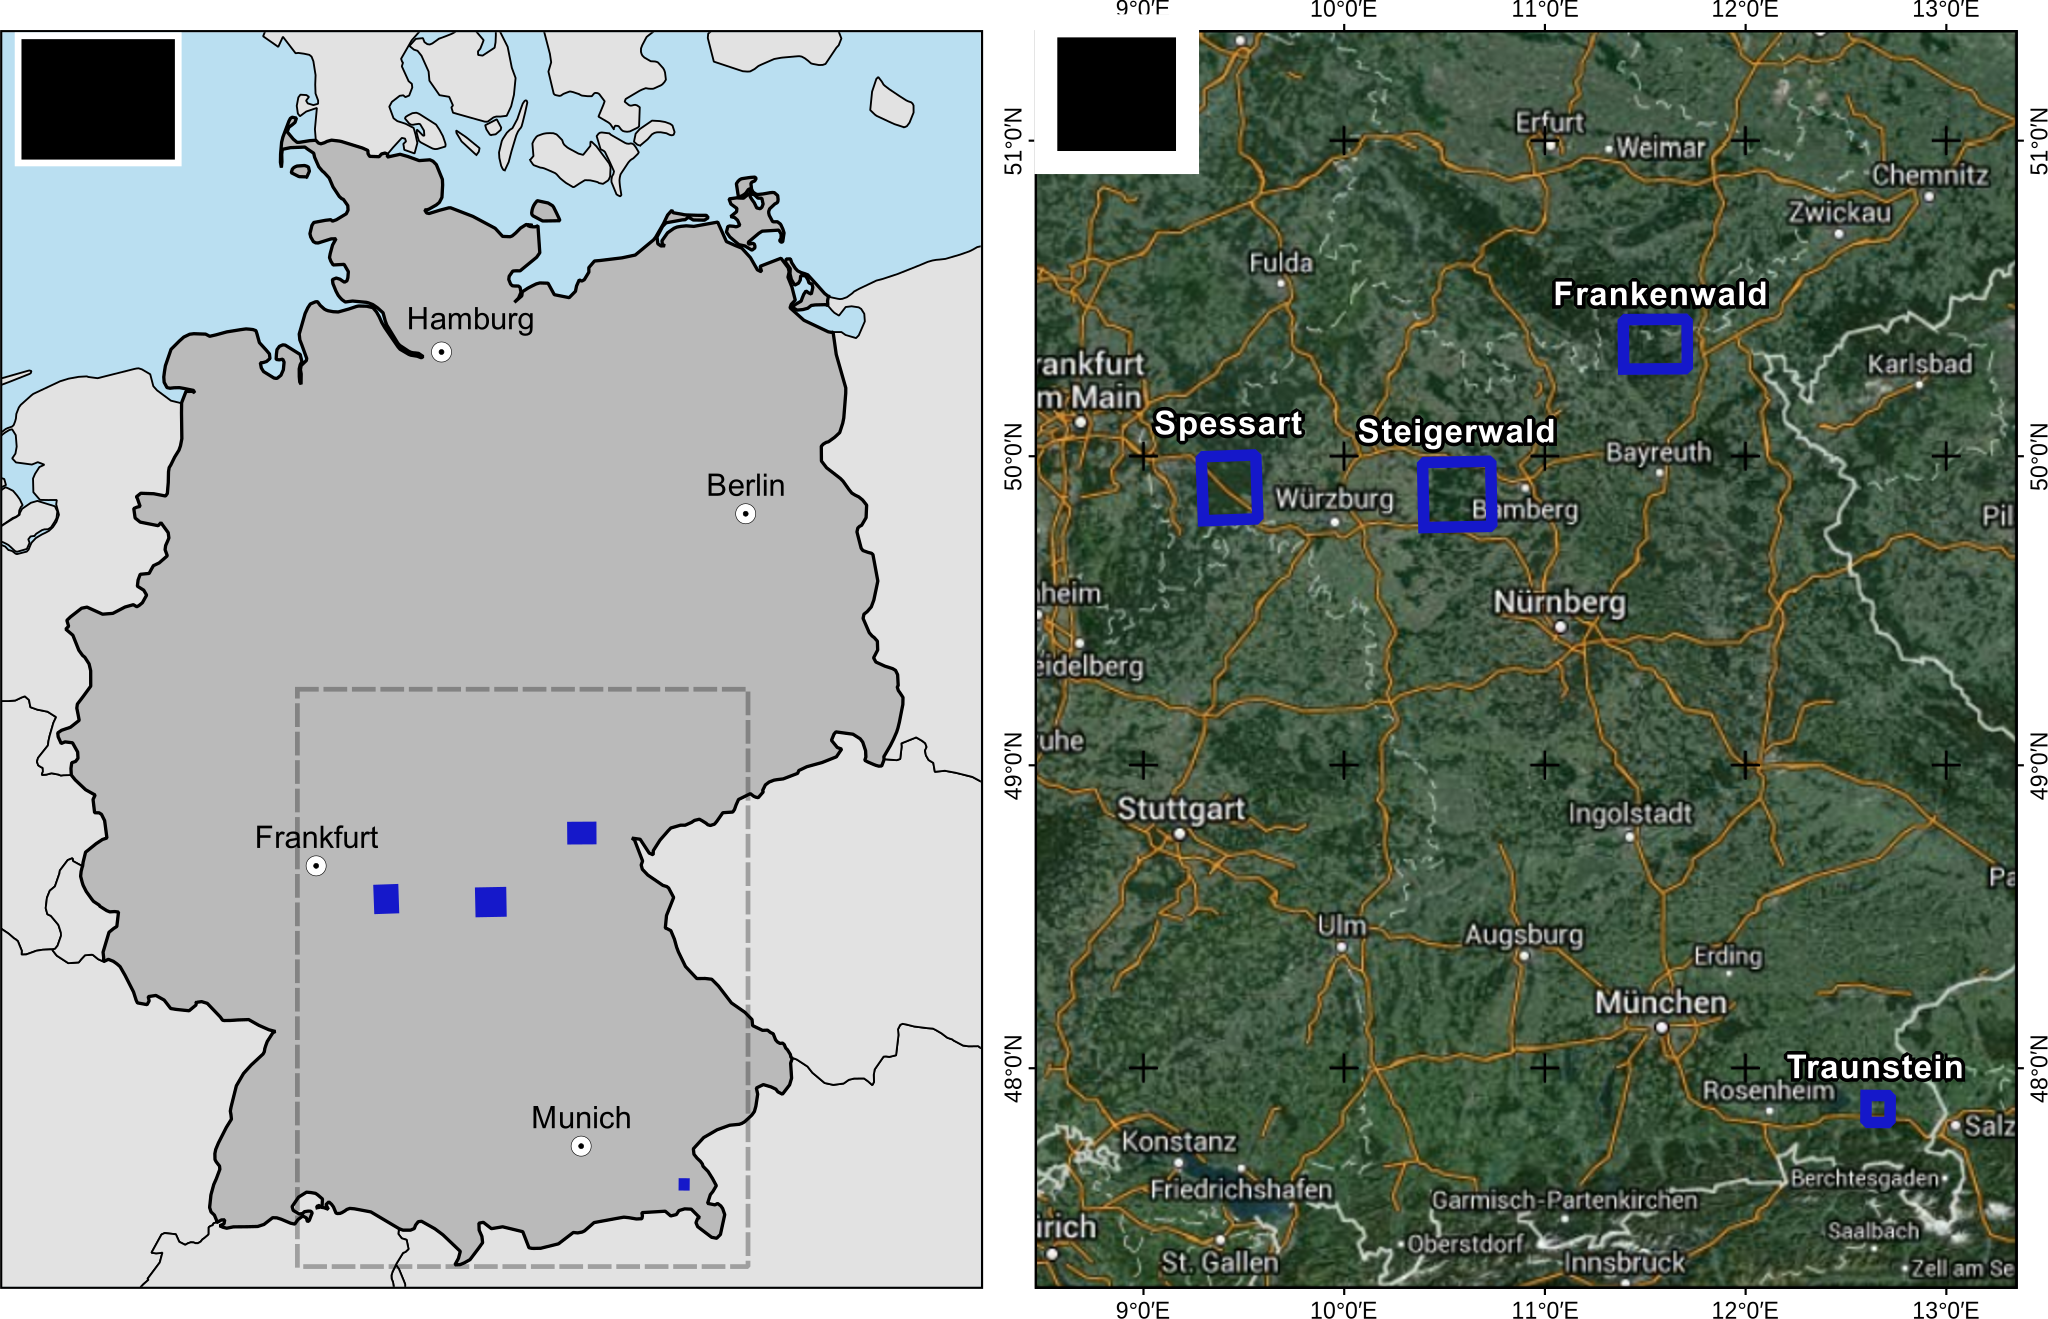
\includegraphics[width=1\textwidth]{Figures/TestSites/Bavaria/TestSites_BY_2} %scale for golden ratio 0.618
	\caption[Map of the study areas in Bavaria.]{Map of the study areas \emph{Spessart}, \emph{Steigerwald}, \emph{Frankenwald}, 
		and \emph{Traunstein} in Bavaria, Germany. (a) Location in Germany; (b) detailed locations in Bavaria 
		(Images \textcopyright Landsat, Mapdata \textcopyright
		GeoBasis-DE/BKG(\textcopyright\,2009), Google).}
	\label{fig:TestSites_BY}
\end{figure}

\begin{figure}[!h]
	\centering
	\includegraphics[width=.9\textwidth]{Figures/TestSites/NVI/wfp_BritishColumbia_testSite} %scale for golden ratio 0.618
	\caption[Map of the study area in British Columbia.]{Map of the study area \emph{Northern Vancouver Island} in 
		British Columbia, Canada. (a) Location in British Columbia, Canada;
		(b) location on \mbox{Northern} Vancouver Island; (c) boundaries of the study area units.}
	\label{fig:TestSite_NVI}
\end{figure}


\section{Field Data}\label{sec:FieldData}

\subsection{Bavarian State Forest Enterprise}\label{subsec:FieldData_BaySF}

Main parts of the test sites \emph{Spessart}\index{study area!Bavaria!Spessart}, \emph{Steigerwald}\index{study area!Bavaria!Steigerwald}, 
and \emph{Frankenwald}\index{study area!Bavaria!Frankenwald} are state-owned\index{state-owned} land, 
mostly managed forests with a great variety of stand development stages. The areas are managed by the 
\ac{BaySF}, and field data are recorded frequently according to their forest management guidelines \parencite{Neufanger.2011}.

For the respective forests, \graffito{Ground plots for terrestrial inventory measurements are permanently marked in the Bavarian state forests.} 
recurring terrestrial sample-based forest inventory systems are installed, and 
comprehensive measurements are carried out on a 10-year frequency basis.
The permanent ground plots where the data are collected are laid out in a regular grid pattern of 200\,m\;x\;200\,m.
The plot centres are permanently marked in the field, and during the inventories, each particular plot location is georeferenced 
using a GPS device. 

The forest management inventories \graffito{Tree measurements at the plots are made according to concentric sampling circles.} 
in the state forests of Bavaria make use of the sampling concept with three concentric measurement circles\index{concentric sampling circles}
at the respective ground plots. A general introduction to this concept can be found in \textcite{vanLaar.2007}. Here, the trees are recorded with 
all relevant attributes in dependency of their \acl{DBH} (\acs{DBH}; measured at 1.3\,m above ground) and their distance to the plot centre.
For the forest inventories conducted by \ac{BaySF}, the radii and \acs{DBH} thresholds for the concentric circles 
assembling a circular inventory plot typically are set as summarized in Table~\ref{tab:Radii}.

\begin{table}[htb]
	\myfloatalign
	\caption[Radii and DBH thresholds for the concentric sampling circles.]{Radii and \ac{DBH} thresholds for the concentric sampling circles
		assembling a ground plot in typical \ac{BaySF} management inventories.}
	\label{tab:Radii}
	\small
	\begin{tabularx}{.8\textwidth}{XXXX}
		\toprule
		\spacedlowsmallcaps{Circle} \linebreak \spacedlowsmallcaps{No.} & \spacedlowsmallcaps{Radius} \linebreak \footnotesize{[m]} & \spacedlowsmallcaps{Area} \linebreak \footnotesize{[m\textsuperscript{2}]} & \spacedlowsmallcaps{DBH} \linebreak \footnotesize{[cm]}  \\ 
		\midrule
		\emph{1} & 2.82 & 25 & $<$\,12  \\ 
		\emph{2} &  6.31 &  125 & 12--29.9 \\
		\emph{3}  & 12.62 &  500 & $\geq$\,30  \\ 
		\bottomrule
	\end{tabularx}
\end{table}
 
Based on the individual tree measurements, \graffito{A set of forest inventory attributes is computed based on the individual tree measurements.}
a set of forest inventory attributes\index{forest inventory attribute} is computed. 
These compiled data sets include, 
inter alia, mean tree height, basal area per hectare, and gross volume per hectare.
In the course of the research project, other attributes, \eg, stand top height, came into focus, 
and procedures were applied to compute the attributes from the individual tree measurements. 

The field data \graffito{Field data in the test sites \emph{Spessart}, \emph{Steigerwald}, and \emph{Frankenwald} were 
	acquired in 2011, 2010, and 2014.} 
for the \ac{BaySF} test sites included in this work, namely \emph{Spessart}, \emph{Steigerwald}, and \emph{Frankenwald},
were recorded in 2011, 2010, and 2014, respectively. 
For more detailed descriptions of the field data acquisitions as well as 
the derivation of forest inventory attributes, refer to the respective sections in the articles. 

\subsection{National forest inventory data}\label{subsec:NFI_data}

Field data from the German \ac{NFI}\index{national forest inventory}\index{NFI|see{national forest inventory}} were selected as reference data for 
model training in the study of \textcite{Immitzer.2016}.
Contrary to the concentric sampling circles used within the management forest inventories of \ac{BaySF},
\graffito{\ac{ACS}\index{angle-count sampling}\index{ACS|see{angle-count sampling}} is used as basic sampling principle in the German \ac{NFI}.} 
the German \ac{NFI} is based on \acf{ACS} as basic sampling principle. Here, the probability of a tree for inclusion to the measurements
is proportional to its basal area at a defined height. Each tree trunk is focused from the sample plot centre and is 
selected if the \ac{DBH} exceeds a prescribed angle width (defined by the so called basal area factor). 
For more information regarding the German \ac{NFI} and the \ac{ACS} method, refer to the corresponding section in the 
paper \parencite{Immitzer.2016} or to \textcite{Polley.2010}.

 Our study was conducted in the \emph{Steigerwald} test site, 
 and a total of 92 sample plots from the most recent \ac{NFI} were used for modelling. 
 \graffito{\ac{NFI} field data were recorded in 2011 and 2012.}The field measurements were conducted in 2011 and 2012, 
 and field-based estimates of growing stock, separately for conifers and broadleaves, 
 were made available to us. 

\subsection{Municipal Forest of Traunstein}\label{subsec:FieldData_Traunstein}

The forest area, which was chosen as test site for the study of \textcite{Stepper.2015}, is part of the municipal forest which belongs 
to the city of Traunstein\index{study area!Bavaria!Traunstein}. 
The forest stands are actively managed to support an uneven-aged mixed-species forest and comprise a 
great variety of successional stages, \ie, heterogeneous species composition, many different age classes, and multi-layered stands.

Similarly to the field sampling design described above for the \ac{BaySF} inventories (subsection~\ref{subsec:FieldData_BaySF}), 
the permanently marked field plots within the \emph{Traunstein} study area -- 228, in total -- are distributed in a regular grid pattern of 100\,m\;x\;100\,m.
At the plots, measurements are carried out using concentric sampling circles\index{concentric sampling circles}, 
based on the following radii and corresponding \ac{DBH} thresholds:
3.15\,m (\ac{DBH}\,$<$\,10\,cm), 6.31\,m (10\,$\leq$\,\ac{DBH}\,$<$\,30\,cm) and 12.62\,m (\ac{DBH}\,$\geq$\,30\,cm).

The \emph{Traunstein} forest test site \graffito{Field measurements collected in 2008 and 2013 were available 
	for the \emph{Traunstein} test site.} was selected for our experiment of assessing forest height changes 
by means of \ac{DAP}-based \acp{CHM}, as field measurements from two terrestrial inventories carried out in 2008 and 2013 were available.
Using the ground plot measurements, field-based top heights were calculated for each inventory plot, and in consequence, field-based
\acf{PAI}\index{periodic annual increment}\index{PAI|see{periodic annual increment}} could be derived as reference for our investigation. 
Details regarding the ground measurements and the subsequent calculations are given
in the respective sections of the paper \parencite{Stepper.2015}.


\subsection{Northern Vancouver Island}\index{study area!British Columbia!Northern Vancouver Island}

To select \graffito{Stratified random sampling was used to select the ground plot locations at \ac{NVI}.}
the ground plot locations in the \ac{NVI} study area, a stratified random sampling\index{stratified random sampling} design was used. 
The ground plots were allocated to five different strata, defined by species information, biogeographic data, and elevation data. 
The sample locations within the strata were selected by a systematic partition, informed by the 3d \ac{ALS}-derived feature space.

In total, 140 ground plots were established within the \ac{NVI} test site (which corresponds to a much greater area representativeness
of the individual plots compared to the ones described in subsections~\ref{subsec:FieldData_BaySF} and~\ref{subsec:FieldData_Traunstein}). 
In the field, the plot centres were established using a GPS device, and all live standing trees with \ac{DBH}\,$\geq$\,12.0\,cm were measured
within a radius of 14\,m ($615.75 m^2$). The individual tree measurements included \ac{DBH}, stem height, age and other mensurational data, 
and estimates for different forest inventory attributes, including Lorey's mean height, basal area, and gross volume, were calculated for each plot
\parencite{White.2015}.


\section{Remote Sensing Data}\label{sec:RemSensData}

This work was purposely designed to investigate digital aerial photographs\index{aerial photograph!digital aerial photograph} 
as remote sensing data for use in forest inventory and management applications. 
Thus, airphotos were the primary remotely sensed data used for analysis in this study.
Besides aerial photography, we examined stereo \acf{WV2}\index{WorldView-2} satellite data for generating 3d height measurements of forest canopies,
and the consequent use for a wall-to-wall mapping\index{wall-to-wall mapping} application of forest inventory data. 
\ac{ALS} data were used twofold: (i)~as indispensable source of information providing detailed elevation models, \ie, ground heights of the terrain; 
(ii)~as reference remote sensing data used in the \ac{ABA}\index{area-based approach} modelling of forest inventory attributes, 
\ie, to judge the achieved results when using 
\ac{DAP} derived height information.

\subsection{Digital Aerial Photographs}

The \graffito{Digital airphotos are acquired routinely by the Bavarian Administration for Surveying.} digital aerial photographs
used for the studies conducted in the Bavarian test sites (see Table~\ref{tab:TestSites}) were provided by the 
Bavarian Administration for Surveying. Currently, the aerial photographs are updated every three years in Bavaria.
General specifications for these official aerial photographs are provided in \textcite{LDBV.2015c}.

All images used in our studies were acquired during leaf-on\index{leaf-on} conditions with digital aerial frame cameras, and both 
panchromatic\index{panchromatic} (PAN) and PAN-sharpened multispectral\index{multispectral} images (blue, green, red, and near infrared) of the same 
radiometric resolution\index{resolution!radiometric} (12\,bit) were available. 
The aerial photographs were acquired such that a \ac{GSD}\index{ground sampling distance} of 0.20\,m  could be ensured for all images.   

The overlaps \graffito{The typical overlaps of the stereo images in Bavaria were 65--75\,\%  in forward and 25--40\,\% in side direction.}
of the stereo images varied between different years of data acquisition and different test sites,
but, in general, overlaps in forward\index{overlap!forward} and side\index{overlap!side} direction of 65--75\,\% and 25--40\,\% were achieved.
For details regarding the used camera type, the individual image overlaps, and the flight dates of the aerial surveys,
the reader is referred to the respective sections of the research articles.

With regard to the study conducted on \ac{NVI}, digital aerial imagery was acquired by the tree farm licensee
Western Forest Products Inc. being responsible for the management of the forests within the study area.
For complete coverage of the area, imagery was acquired during four different flights from August to October 2012.
The photographs were acquired with a minimum of 60\,\% along-track (forward) and 20\,\% across-track (side) overlap.
The airphotos were provided as 4-band (blue, green, red, near infrared) multispectral\index{multispectral} images with a 0.30\,m \ac{GSD} and 
8\,bit radiometric\index{resolution!radiometric} resolution.

\subsection{World-View 2 Data}

In the study of \textcite{Immitzer.2016} we explored the usability of high-resolution optical satellite imagery\index{optical satellite imagery} 
recorded in stereoscopic collection mode for the image-based generation of 3d height data and further application. 
Therefore, \ac{WV2} stereo satellite image data were used.
\ac{WV2} records panchromatic\index{panchromatic} images plus multispectral\index{multispectral} images 
comprising eight spectral bands (coastal, blue, green, yellow,
red, red edge, near infrared~1, near infrared~2; \cite{DigitalGlobe.2013}).
 
For the test site \emph{Steigerwald} complete coverage was achieved through two stereo-image pairs, \ie, four \ac{WV2} images,
which were recorded under leaf-on\index{leaf-on} conditions in August 2013. The spectral data were atmospherically corrected and thus, top-of-canopy
spectral reflectance was available for further analysis. 
The \ac{WV2} data were provided as panchromatic images with 0.50\,m spatial\index{resolution!spatial} resolution, 
and as 8-band multispectral images resampled to 1.0\,m pixel size.

\subsection{Airborne Laser Scanning Data}

As mentioned above, one essential benefit of \ac{ALS}\index{airborne laser scanning} 
data sets is that measurements describing the canopy structure and the ground surface 
can be acquired simultaneously. This allows for the computation of vegetation heights using inherent ground measurements.
For the \ac{DAP}-based reconstruction of vegetation height, additional bare earth information is necessary. 

The Bavarian Administration for Surveying routinely runs \ac{ALS} mapping surveys in order to achieve accurate measurements of the terrain
(however, with no distinct repeat cycle).
Based \graffito{\acp{DTM} with 1\,m ground resolution are available for the entire area of Bavaria.}
on these \ac{ALS} data, \acfp{DTM}\index{DTM|see{digital terrain model}}\index{digital terrain model} with 1\,m ground resolution
are available for the entire area of the country \parencite{LDBV.2015b}.
In the course of the research project, the \ac{ALS}-based \acp{DTM} were used for the height normalization\index{height normalization} 
of the \ac{DAP}-based surface measurements.
Canopy heights were consequently calculated as difference of the image-based surface heights and the \ac{ALS}-based terrain heights.

In the \ac{NVI} study area \ac{ALS} point clouds\index{point cloud} were acquired at the same time as the digital airphotos, \ie, in August and September 2012. 
The data had an average return point density\index{point density} of 11.6\,points$\cdot$m\textsuperscript{2}.
Based on the ground returns from that data, a \ac{DTM} with a spatial resolution of 1\,m was created. The \ac{DTM} was used to normalize the 
\ac{ALS} point cloud heights to heights above ground level. In addition, the image-based points from the \ac{NVI} study area were transformed to heights
above ground using the same \ac{ALS}-based \ac{DTM}. 


 
    


%************************************************
\chapter{Methods}
\label{chp:Meth}
%************************************************

\section{Digital aerial photogrammetry}\label{sec:DAP}

\subsection{General Considerations on Image Matching}

Photogrammetry\index{photogrammetry} \graffito{3d coordinates of objects can be derived from stereo images via photogrammetry.} is a measurement technique
to derive 3d\index{three-dimensional} coordinates of object points, which are depicted on 
images taken from different positions \parencite{Lemmens.2011b}.
By utilizing the stereophotogrammetric measuring principle (see subsection~\ref{subsec:HeighAssessStereo}) 
and with known orientation\index{image orientation} parameters of the images\footnote{\emph{interior orientation:}\index{image orientation!interior orientation} 
	focal length, principal point ($X, Y$), pixel size;
	\emph{exterior orientation:}\index{image orientation!exterior orientation} position coordinates of the projection centre ($X, Y, Z$), 
	plus angular parameters ($\omega, \phi, \kappa$).},
 the coordinates of the objects of interest can be retrieved via triangulation\index{triangulation}.
According to \textcite[p. 231]{Schenk.1999}, 

\begin{quote}
”[o]ne \graffito{Identification and measurement of conjugate points in overlapping images is fundamental in photogrammetry.}
of the most fundamental processes in photogrammetry
is to identify and to measure conjugate
points in two or more overlapping photographs.
Stereo photogrammetry relies entirely on conjugate
points. In analogue and analytical photogrammetry
the identification of conjugate points
is performed by a human operator; in digital photogrammetry
one attempts to solve the problem
automatically -- a process known as image matching\index{image matching}.”
\end{quote}

\noindent The introduction of stereo-image matching techniques in photogrammetry allowed for automation in different processing steps, 
particularly in the creation of dense height measurements, and is the fundamental basis for \ac{DAP}.
Generally speaking, the aim of image matching is to identify corresponding pattern in the stereo-image pairs, 
\ie, the base and the match image. The problem in finding these correspondences is to trace and locate the pattern 
in the match image as the conjugate of a pattern in the base image \parencite{Lemmens.2011b}.

Traditionally, the image-matching methods \graffito{Established image matching categories: \emph{feature-based} and \emph{area-based} matching.}
may be assigned to two categories depending
on how the image -- an array of pixels storing digital numbers -- is approached \parencite{ERDAS.2010, Gruen.2012}.
The first category can be classified as \emph{feature-based matching} approaches\index{image matching!feature-based matching}. 
These focus on the evaluation of similarities 
of extracted features in both base and match image, which may be depictions of prominent features like corners of buildings, road crossings,
or solitaire trees in case of aerial photographs.
The second group of algorithms can be categorized as \emph{area-based matching} approaches\index{image matching!area-base matching}.
Here, correspondence between the stereo images is sought using the grey level values in regularly shaped patches, \eg, 9\,x\,9\,pixel windows. 
A reference window, remaining at a constant location in the base image, is defined as source for calculating correlation to 
candidate windows on the match image. Many different search windows in the match image are evaluated until the location for correspondence is
determined by the highest value for the correlation coefficient. 
Consequently, the centre pixels of the reference and search window are selected as corresponding points.
Most commonly, normalized cross-correlation (NCC)\index{normalized cross-correlation} is used for calculating correlation and acceptance of the match 
depends on whether the similarity value exceeds a predefined threshold \parencite{Lemmens.2011b}. 
A trade-off is associated with the definition of the correlation threshold: whereas choosing too small values allows for many mismatches, \ie,
wrong correspondences of pixels, too high values impede many matches and in consequence, the density of matches found for a stereo-image pair decreases.

\subsection{Semi-global Matching}\index{semi-global matching}

Problems with finding correspondences are especially connected to object boundaries, fine structures, low and repetitive textures, and recording
and illumination differences in the images.
In order to overcome these drawbacks, effort was put into developing new image-matching methods.
One approach which have gained considerable attention in recent years, is the so-called \acf{SGM} technique\index{SGM|see{semi-global matching}} introduced by \textcite{Hirschmuller.2005,Hirschmuller.2008}.
\ac{SGM} is based on the idea of pixelwise matching\index{image matching!pixelwise matching} and approximating a global 2d smoothness constraint by combining 
many 1d constraints.
The basic steps of \ac{SGM} are:
\begin{itemize}
	\item Generation of epipolar images\index{epipolar images} by projectively warp the base and match images with known geometries 
		such that the epipolar lines are horizontal.
	\item Calculation of possible disparities\index{disparity} for each pixel along the epipolar search lines in the base image and computation of 
		matching costs\index{matching cost} for each candidate disparity by a similarity measure (\eg, Mutual Information, Census) comparing the pixel grey values. 
	\item Aggregation of costs by pathwise accumulation of minimal costs along a certain number of 1d path directions through the base image.
		Here, additional smoothness constraints are introduced by penalizing disparity changes.
	\item Determination of final disparities for each pixel in the base image by selecting the candidate pixel in the match image 
		that corresponds to the minimum cost.
	\item Intersection of viewing rays in the stereo images according to the final disparity image to achieve 
	dense 3d\index{three-dimensional} point clouds\index{point cloud} in object space. 
\end{itemize}
More details regarding the performed steps in \ac{SGM} and the implemented algorithms are provided in, \eg, \textcite{Hirschmuller.2008,Hirschmuller.2011} and \textcite{Gehrke.2010}.

We applied the \ac{SGM} approach for image matching\index{image matching} and consecutive derivation of image-based surface heights throughout the studies
presented in this work\footnote{except for \textcite{Immitzer.2016}: here, the area-based normalized cross-correlation method implemented 
	in LPS eATE (ERDAS IMAGINE 2014) was used.}. 
For the processing, we used the \ac{SGM} implementation within the Remote Sensing Software Package Graz (RSG).
The cost function used in RSG follows the Census disparity measure, and 
the matching procedure is hierarchically structured as coarse to fine matching, with consequent disparity calculations on four image pyramid levels. 

We selected the panchromatic\index{panchromatic} band \graffito{Panchromatic images were used for matching of along-track stereo-image pairs covering the Bavarian test sites.}
of the stereo images for matching in all Bavarian test sites. Due to the low across-track overlaps of the images,
we used only stereo-image pairs from the along-track overlap for calculation.
For the \ac{NVI} test site, the airphotos were only available as multispectal\index{multispectral} images (\emph{RGBI}). Here, the green band was selected for matching.

As outputs from dense stereo matching in RSG, we opted for using the raw dense 3d point clouds from the respective stereo pairs and used additional utility software for 
further processing. In the work concerned with the assessment of height changes \parencite{Stepper.2015}, 
we used \acp{DSM}\index{digital surface model}\index{DSM|see{digital surface model}} as outputs from the RSG streamline for further analysis.
  
The products from \ac{DAP}, \ie, the dense image-based point clouds or the \acp{DSM}, were further processed to calculate the object heights above ground 
by using the \ac{ALS}-based elevation heights for subtraction. 
Subsequently, different data processing steps (clipping to inventory point geometries, etc.) were performed in order to prepare appropriate data sets for 
consequent use in statistical modelling. Details regarding the particular processing steps are given in the respective paper sections.
 

\section{Statistical Modelling}\label{sec:StatModel}

As introduced in sections~\ref{sec:AerialPhotogrammetry} and~\ref{sec:ABA},
the \acf{ABA} gained strong interest for integrating remote sensing data sets, in particular \ac{ALS} and \ac{DAP}-based products,
for use in forest inventory and mapping applications.

% long sentence, maybe split into two shorter!
In this context, \ie, for the combination of ground based measurements and the remotely sensed data, statistical models which can produce
unbiased and accurate estimates of the forest attribute\index{forest inventory attribute} of interest by means of remote sensing predictor variables\index{predictor variable}
play a key role. 
In the \ac{ABA}\index{area-based aproach} workflow (see Figure~\ref{fig:ABA_method}), the statistical models are trained with known samples, 
namely the ground-based inventory measurements and the descriptive statistics (\mbox{\emph{metrics}}) calculated 
from the remote sensing data clipped to the areas of the georeferenced inventory plots --
and consequently, these models are applied to predict estimates over entire forest areas.

Therefore \graffito{The statistical model describes the dependency between the remote sensing predictors and the ground-based response.}
it is crucial, that the chosen model type is able to accurately map the statistical dependency between the remote sensing predictor variables
and the response variables\index{response variable} derived from the ground measurements (\eg, mean stand height or volume).
In the literature, different regression\index{regression model} approaches (parametric\index{regression model!parametric} 
and non-parametric\index{regression model!non-parametric}) were applied to fulfil this task. 
Besides linear regression modelling, the decision-tree based approach \acf{RF}\index{regression model!non-parametric!random forest} 
was most widely used for predictive modelling of 
forest inventory attributes through the course of the presented studies.
Therefore, and without judging other approaches for their appropriateness, the main characteristics of \ac{RF} and its actual application are described.

\subsection{Random Forest for Regression}

\ac{RF} can be assigned to \graffito{\ac{RF} requires no a priori assumption about the relationship of predictors and response variables.}
the domain of non-parametric modelling approaches.
Thus, no \emph{a priori} assumptions about relationships between predictor\index{predictor variable} and response variables\index{response variable} 
are made \parencite{White.2013}.
Due to that, and to the fact that very little tuning is required during model building, \ac{RF} has become a popular method in predictive modelling.

\ac{RF}, developed by \textcite{Breiman.2001}, is an ensemble regression tree algorithm (see Algorithm~\ref{algo:RF}) based on a 
large collection of \emph{de-correlated} decision trees\index{regression model!non-parametric!decision tree} \parencite{Hastie.2009}. 
\ac{RF} \graffito{An ensemble of de-correlated decision trees forms a \ac{RF} model.}
can be seen as further development of bagging (\emph{bootstrap aggregation}), as the individual trees that constitute the forest are 
fitted to bootstrap-sampled versions of the training data, and averaged to get the final result
(for a schematic of \emph{bootstrap sampling}, see Figure~\ref{fig:bootstrap}).

In \ac{RF}, a second randomization is introduced to the tree-building process, in order to additionally reduce the correlation between the trees: 
the algorithm randomly selects a subset of predictor variables as candidates for splitting at each decision node.
\ac{RF} has two potential parameters for adjustment: 
(a)~the number of randomly selected predictors \emph{m}, from which to choose at each split 
(commonly referred to as $m_{\textsf{try}}$). 
For use in regression, the algorithm inventor \citeauthor{Breiman.2001} recommended $p/3$ as default value, \ie, one third of the 
number of predictors \parencite{Breiman.2001}; (b) the number of trees in the forest (commonly referred to as $n_{\textsf{tree}}$). 
As \ac{RF} is not prone to over-fitting, large numbers of trees do not adversely affect the model accuracy. 
However, the computational expense increases. \textcite{Kuhn.2013b} suggest 1\,000 trees as starting point,
and adjustment in dependence of the achieved model performance.
Important advances and features of \ac{RF} are:

\begin{description}
	\item[distribution independence] The variables ($x, y$) used as predictors and response in modelling do not have to follow a predefined distribution.
	\item[dimensionality] In \ac{RF}, high-dimensional and highly correlated data sets can be processed without suffering a loss in performance.
	\item[\acf{oob}]\index{out-of-bag} For each observation $z_i = (x_i, y_i)$, its random forest predictor can be computed by averaging only those trees corresponding to 
		bootstrap samples in which $z_i$ is not included (see Figure~\ref{fig:bootstrap}). 
		Doing so, an \ac{oob} error estimate is almost identical to that obtained by
		N-fold cross-validation (cf. \cite{Hastie.2009}). 
		Thus, performance measures can be computed along the way during \ac{RF} model training.
	\item[variable importance] Information on the importance of each predictor variable used in model building can be computed twofold: 
		(a) as measure of the total decrease in node impurities from splitting on each variable, averaged over all trees; 
		(b) as mean decrease of prediction accuracy, when permuting the values of the predictor variables in the \ac{oob} samples, again averaged over all trees. 
\end{description}



\begin{figure}[tb]
	\centering
	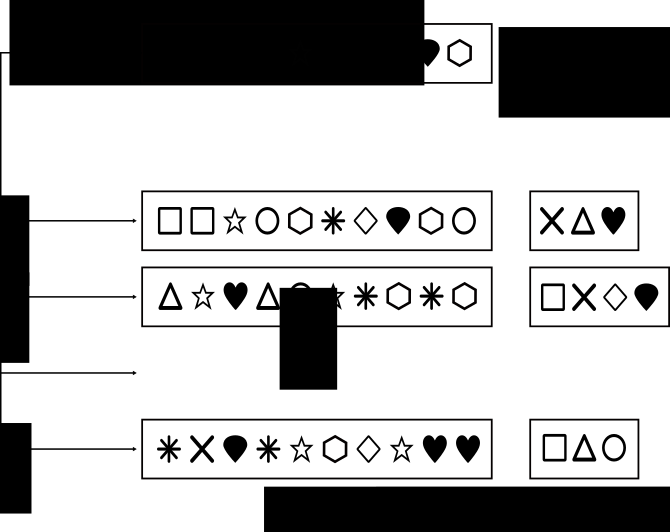
\includegraphics[width=.8\textwidth]{Figures/bootstrap/bagging_RF_landscape} %scale for golden ratio 0.618
	\caption[Schematic of bootstrap resampling used in Random Forests.]
	{Schematic of bootstrap resampling as used in \ac{RF} for drawing the training samples for the individual regression trees.
		The training sample data are depicted as symbols and are allocated to \emph{B} subsets, each taken as random sample \emph{with replacement}.
		The subsets are of the same size as the original training data and can contain multiple instances of the same data point. Samples not selected by the
		bootstrap\index{bootstrap} are the \emph{out-of-bag}\index{out-of-bag} data and can be used to estimate model performance (modified after \cite{Kuhn.2013b}).}
	\label{fig:bootstrap}
\end{figure}



\begin{algorithm}[bt]
	\SetAlCapFnt{\small\sffamily\bfseries}
	\SetAlCapNameFnt{\small}
	\small
	%\TitleOfAlgo{test}
	%\SetAlgoLined
	\DontPrintSemicolon
	
	Select the number of trees to build, \emph{B}:\;
	\BlankLine
	\For{b = 1 to B:}{
		(1) Draw a bootstrap sample \textbf{Z*} of size \emph{N} from the training data.\;
		(2) Train a tree model $T_b$ to the bootstrapped data, by recursively repeating the following steps for each terminal node of the tree,
		until the minimum node size $n_{\textsf{min}}$ is reached.\;
		\For{each split:}{
			(a)\:Select \emph{m} variables at random from the \emph{p} predictor variables (\emph{m}\,$\leq$\,\emph{p}).\;
			(b)\:Pick the best variable/split-point among the \emph{m}.\;
			(c)\:Split the node into two data nodes.
		}
	}
	\BlankLine
	Output the ensemble of trees $\left\lbrace T_b\right\rbrace _1^B$.\;
	\BlankLine
	To make a prediction at a new point \emph{x}:\;
	$\hat{f}_{rf}^B(x)=\frac{1}{B}\sum_{b=1}^B T_b(x)$
	
	\caption{Random Forest for Regression (modified after \cite{Hastie.2009} and \cite{Kuhn.2013b}).}
	\label{algo:RF}		
\end{algorithm}


\subsection{Model Implementation for predicting Forest Inventory Attributes}\index{forest inventory attribute}

We used functionalities and add-on packages of the open-source statistical software \textsf{R} to accomplish all statistical tasks.
For model development (using the data gathered at the forest inventory plots) and prediction to unknown samples by means of \ac{RF},
the functionalities provided in the packages \textsf{caret} \parencite{Kuhn.2015} and \textsf{randomForest} \parencite{Liaw.2002} were principally used. 
 
With regard to the tuning parameters of \ac{RF}\index{random forest}, we followed the recommendation of \textcite{Kuhn.2013b}: 
The number of regression trees in the respective forests was set to $n_{\textsf{tree}} = 1000$, 
and the number of variables randomly selected at each split was set to $m_{\textsf{try}} = p/3$.

In all studies, the \acf{RMSE}\index{RMSE|see{root mean squared error}}\index{root mean squared error} and 
\acf{ME}\index{ME|see{mean error}}\index{mean error} measures were selected to evaluate model performance, \ie, model accuracy\index{accuracy} and bias\index{bias}.
In the studies of \textcite{Stepper.2015b,White.2015,Straub.2016}, we applied a 10-fold cross-validation\index{cross-validation} repeated five times to assess model performance
and in the studies of \textcite{Immitzer.2016,Stepper.2016} the \ac{oob}-estimates\index{out-of-bag} were used for model evaluation.

Additionally, the model performance at the stand level, \ie, after wall-to-wall prediction mapping and aggregating to forest stands, 
was examined in the studies of \textcite{Stepper.2015b, Immitzer.2016}.
Independent inventory data from nearby forests were utilized to assess model transferability in the study of \textcite{Stepper.2016}, 
again by means of \ac{RMSE} and \ac{ME}.
For more details regarding model training and evaluation, the reader is referred to the respective articles. 


\section{Height Change Assessment}\label{sec:HeightChange}

Elaborating on the aim to test the utility of digital stereo images from repeat surveys for forest height change assessment,
we developed a workflow as illustrated in Figure~\ref{fig:meth_heightChange}.

\begin{figure}[!b]
	\centering
	\includegraphics[width=1\textwidth]{Figures/heightChange/Method_heightChange} %scale for golden ratio 0.618
	\caption[Methodological workflow for height change assessment using terrestrial measurements and image-based CHMs.]
	{Methodological workflow for height change assessment using terrestrial measurements and \acp{CHM}\index{canopy height model}\index{CHM|see{canopy height model}} 
		based on stereo airphotos from repeat aerial image surveys. \textbf{(a)} Terrestrial assessment: 
		(1) tree crown heights are measured for representative samples at the respective inventory plots, 
		(2) top heights ($H100$) are modelled using the height measurements of trees from the overstory and emergent tree layers, 
		(3) \ac{PAI}\index{periodic annual increment}\index{PAI|see{periodic annual increment}} is calculated as the difference between 
		the modelled $H100$ values for
		the two inventory dates divided by the time lapse between the two inventories. 
		\textbf{(b)} Aerial image assessment: 
		(1) digital stereo images are acquired in regularly scheduled aerial surveys, 
		(2) \acp{CHM} are created by subtracting \ac{LiDAR}-derived terrain heights from image-based surface models, 
		(3) \ac{PAI} is computed as the difference between the maximum height
		values ($h_{max}$) from the two \acp{CHM} divided by the time lapse between the two image dates.}
	\label{fig:meth_heightChange}
\end{figure}

We followed the \ac{SGM}\index{semi-global matching} approach (see section~\ref{sec:DAP}) to accomplish image matching\index{image matching} of the stereo airphotos. 
In our study \parencite{Stepper.2015},
we chose the RSG software utilities for image matching and used the implemented functionality to output \acp{DSM} with 1\,m resolution for both dates of image acquisition.
Finally, \acp{CHM} were derived by subtracting the elevation values of the bare earth \ac{DTM} from the z-values of the two \acp{DSM}.

Terrestrial inventory measurements, acquired for circular 500\,m\textsuperscript{2} plots, 
were used as reference for the assessment of forest canopy height and height changes.
$H100$ was calculated from the field measurements as height metric approximating top heights of forest stands. In our study, $H100$ was 
defined as the average height of the 100 stems per hectare with the largest \acp{DBH} (see \emph{Algorithm~1} in the article for the explicit computation rule set). 

To link the \ac{CHM}-heights with the field-based $H100$ top heights, various height percentiles (25th, 50th, 75th, 90th, 95th, and maximum) were calculated
from the \ac{CHM}-values for the areas within each of the 500\,m\textsuperscript{2} circular plots.
The percentiles\index{percentile} were correlated to the field-based top heights and 
the maximum height of the \ac{CHM} ($h_{max}$) turned out to achieve highest correlation values.
Thus, this variable was selected for the height change assessment.

Height differences between the two points in time from the terrestrial and the aerial image acquisitions were used to calculate \acfp{PAI} as 
standardized increment measures per unit of time (see Figure~\ref{fig:meth_heightChange}).
The \acp{PAI}, both from the field measurements and the image-based height data, were regressed against the $H100$ top height values based on the 
initial field data (from $t_{1,\textsf{field}}$) to analyse the relationship between initial forest height and height growth.
Finally, differences between increments for initial height classes representing various forest successional stages were examined.  



%************************************************
\chapter{Results}
\label{chp:Results}
%************************************************

The results of the conducted research were published in different scientific papers. In the following, the papers are summarized and the personal contribution is highlighted. 


\section{Paper 1}\label{sec:Paper1}

Title: Using semi-global matching point clouds to estimate growing stock at the plot and stand levels: application for a broadleaf-dominated forest in central Europe 

Authors: Christoph Stepper, Christoph Straub, Hans Pretzsch

Journal: Canadian Journal of Forest Research

Journal Impact Factor (2014): 1.683 

Abstract: 

Contribution:



\section{Paper 2}\label{sec:Paper2}

Title: Using digital aerial photogrammetry and the Random Forests approach to model forest inventory attributes in beech- and spruce-dominated central European forests

Authors: Christoph Straub, Christoph Stepper

Journal: Photogrammetrie Fernerkundung Geoinformation (under review)

Journal Impact Factor (2014): 0.733

Abstract:

Contribution:



\section{Paper 3}\label{sec:Paper3}

Title: Canopy heights from digital aerial photogrammetry to spatially transfer forest attribute models: a case study in central Europe

Authors: Christoph Stepper, Christoph Straub, Markus Immitzer, Hans Pretzsch

Journal: Scandinavian Journal of Forest Research (submitted)

Journal Impact Factor (2014): 1.537

Abstract:

Contribution:



\section{Paper 4}\label{sec:Paper4}

Title: Comparing ALS and image-based point cloud metrics and modelled forest inventory attributes in a complex coastal forest environment

Authors: Joanne C. White, Christoph Stepper, Piotr Tompalski, Nicholas C. Coops, Michael A. Wulder

Journal: Forests

Journal Impact Factor (2014): 1.449

Abstract:

Contribution:



\section{Paper 5}\label{sec:Paper5}

Title: Use of WorldView-2 stereo imagery and National Forest Inventory data for wall-to-wall mapping of growing stock

Authors: Markus Immitzer, Christoph Stepper, Sebastian Böck, Christoph Straub, Clement Atzberger

Journal: Forest Ecology and Management

Journal Impact Factor (2014): 2.660

Abstract:

Contribution:



\section{Paper 6}\label{sec:Paper6}

Title: Assessing height changes in a highly structured forest using regularly acquired aerial image data 

Authors: Christoph Stepper, Christoph Straub, Hans Pretzsch

Journal: Forestry

Journal Impact Factor (2014): 2.093

Abstract:

Contribution:
%************************************************
\chapter{Discussion}
\label{chp:Discussion}
%************************************************

% This is a combining discussion for the different aspects presented in the scientific papers above.

Different aspects of utilizing digital airphotos and height measurements derived thereof by means of \ac{DAP} 
for forest inventory and forest management were considered in the studies presented in this thesis.
Overall, the results confirm that image-based point clouds and \acp{CHM} are a viable source of information
to characterize the three-dimensional structure of forest canopies, at least for the forest types examined
in the different studies (see Table~\ref{tab:TestSites}).

The primary motivations for initiating this work were:
\begin{itemize}
%	\item the growing interest of forest professionals in the use of high spatial resolution \ac{DAP} to generate 
%		3d information to support forest inventory and monitoring \parencite{White.2016}.
	\item the need for spatially explicit information on the current state of forest stands in order to facilitate forest management practice;
	\item the unexploited potential of using digital aerial photographs for the three-dimensional characterization of forest canopies;
	\item the recently launched algorithms to process stereo airphotos to generate image-based height measurements covering large areas;
	\item the possibility to test the \ac{DAP}-based height measurement as surrogate for \ac{ALS}-based data when spatially predicting forest inventory attributes.  
\end{itemize} 


As mentioned in the introduction, large parts of the theoretical framework on using 3d information in forest inventory
were developed based on \ac{ALS} data (\eg, \cite{Naesset.2002b}).
Meanwhile, airborne imaging technologies (\eg, digital cameras) and image processing algorithms and software (\eg, \ac{SGM}) 
have emerged that enable workflows possible to generate image-based point clouds and \acp{DSM} covering large areas \parencite{White.2016}.
Those 3d measurements achieve similar degrees of detail for forest canopy surfaces as the airborne \ac{LiDAR}-based measurements,
and with the large-scale availability of \ac{ALS}-based \acp{DTM}, canopy heights above ground can be derived from 
the photogrammetric data with little additional effort. 

\medskip

\begin{itemize}
	\item Schwerpunkt der Studien: Mitteleuropäische Waldverhältnisse --> Ergebnisse für Schätzung wichtiger Forstlicher Kennzahlen ok
	\item Vergleich mit LiDAR in Canada --> DAP Daten sind ein sinnvolle Ergänzung zu Laser Scanning Daten --> Ermöglichen neue Inventurfortschreibungsverfahren
	 --> viel billiger als Lidar \\ --> regelmäßige Befliegung \\ --> zusätzliche Verfügbarkeit der Spektralen Information
\end{itemize}

\medskip
\begin{itemize}
	\item Wie genau lassen sich die verschiedenen forstlichen Parameter mit der gewählten Methode abschätzen?
	\item auf die unterschiedlichen Kennzahlen eingehen. 
	\item Holzvolumen --> nächste Schritte: Einzelbaum-Verfahren / Durchmesserverteilung approximieren
	\item stärkere Integration der spektralen Kennwerte in die Modellierung (evtl. auch Verwendung von hochaufgelösten Satellitendaten (Phänologie), um Tree species unterscheidbar zu machen)
	\item was waren die wichtigsten Prädiktoren für die unterschiedlichen forstlichen Parameter --> Vergleich der Studien --> allgemeingültige Aussage möglich? Tendenzen? Vergleich mit Lidar?
	\item untersucht: Wie verhalten sich die Modelle in nadel- bzw. laubdominierten Wäldern! Frankenwald vs. Spessart/Steigerwald // Mischwald (Wald der Zukunft) --> Traunstein?
	\item ungelöste Aufgaben: Aussagen über die Baumarten-spezifischen Angaben (z.b. Holzvorrat Nadelbäume vs. Holzvorrat Laubbäume)
 	
\end{itemize}










% a now and emerging area of research is the generation and exploration of 3d information from airborne imagery,
% which has been enabled by recent advances in cameras and computing technologies.



%************************************************
\chapter{Conclusion}
\label{chp:Conclusion}
%************************************************

% A short conclusion to summarize the presented methods, results, and discussion.

The presented methods and achieved results from the different studies approved the high potential
of \ac{DAP} for use in forest inventory and monitoring tasks.
In the studies, image-based height data were employed in combination with different field-measured information sources
(\aclp{MFI}, \acl{NFI}) on a range of spatial scales.
Additionally, due to the lower acquisition costs compared to \ac{ALS}, and the high recurrence frequency of the 
administrative aerial surveys, airphotos and derived \ac{DAP} products
can provide an important bridge between the operational, tactical, and strategic forest management levels. 

The studies confirmed that \ac{DAP}-based height information can be used in conjunction with ground-based measurements 
to establish predictive models for a set of forest inventory attributes \parencites[see][]{Stepper.2015b, White.2015, Straub.2016, Stepper.2016}.
Similar to \ac{ALS}, the most predictive canopy metrics derived from the \ac{DAP}-based measurements were height metrics, 
which are most appropriate to describe the canopy \emph{growing space}. 
It could be demonstrated, that the intra-metric correlation is higher for the image-based data compared to the \ac{ALS} data \parencite[see][]{White.2015},
indicating that it is sufficient for modelling to work with a subset of the computed metrics. 
In \textcite{Stepper.2015b} we could show, that \dots



\begin{itemize}
	\item Baumartenklassifikation ?!?
	\item UAV?
\end{itemize}

\end{linenumbers}

% *****************************************************************
% Backmatter
%******************************************************************

\appendix
%\renewcommand{\thechapter}{\alph{chapter}}
\cleardoublepage
\part{Appendix}
%********************************************************************
% Appendix
%*******************************************************
% If problems with the headers: get headings in appendix etc. right
%\markboth{\spacedlowsmallcaps{Appendix}}{\spacedlowsmallcaps{Appendix}}
\chapter{Appendix}

The complete \graffito{Complete copies of the published and submitted studies.} copies of the published and submitted studies 
are given in the following sections of the appendix. 
They are presented according to the order in Chapter~\ref{chp:Results}, an overview is given in Table~\ref{tab:steppchr_papers}.

\begin{table}[h]
	\myfloatalign
	\caption[Overview of published research papers.]{Overview of published research papers.}
	\begin{tabularx}{\textwidth}{llX} \toprule
		\tableheadline{Authors} & \tableheadline{Year} & \tableheadline{Title}  \\ 
		\midrule
		Stepper et al. & 2015 & Using
		semi-global matching point clouds to estimate growing stock at the
		plot and stand levels: application for a broadleaf-dominated forest in
		central Europe \\
		Straub \& Stepper & in press & Using digital aerial
		photogrammetry and the Random Forests approach to model forest
		inventory attributes in beech- and spruce-dominated central European
		forests \\
		Stepper et al. & subm. & Using
		canopy heights from digital aerial photogrammetry to enable spatial
		transfer of forest attribute models: a case study in central Europe \\
		White et al. & 2015 & Comparing ALS and Image-Based Point
		Cloud Metrics and Modelled Forest Inventory Attributes in a Complex
		Coastal Forest Environment \\
		Immitzer et al. & 2016 & Use of WorldView-2 stereo imagery and Na-
		tional Forest Inventory data for wall-to-wall mapping of growing stock \\
		Stepper et al. & 2015 & Assessing
		height changes in a highly structured forest using regularly acquired
		aerial image data \\
		\bottomrule
	\end{tabularx}
	\label{tab:steppchr_papers}
\end{table}

\cleardoublepage


%\section{Stepper et al. (2015); Can. J. Forest Res.}
%%Add pdf of first paper here.
\includepdf[page={1-}, offset=1cm 0cm, pagecommand={}, 
			clip, trim=1cm 0cm 0cm 0cm, scale=.9, addtotoc={1,section,1,{Stepper et al. \emph{Can. J. For. Res.} (2015) },
			pub.CanJForRes}]{Articles/Stepper2014_SGM_point_clouds.pdf}
		
\nocite{Austin.2004}\nocite{Bohlin.2012}\nocite{Breidenbach.2010b}\nocite{Breiman.2001}\nocite{Everitt.2011b}\nocite{Genuer.2008}\nocite{Gobakken.2008}\nocite{Haala.2011}\nocite{Haala.2013b}\nocite{Haala.2012}\nocite{Haralick.1973}\nocite{Hastie.2009}\nocite{Hawbaker.2009}\nocite{Hirschmuller.2008}\nocite{Hirschmuller.2011}\nocite{Holmgren.2004}\nocite{Holopainen.2013}\nocite{Hudak.2008}\nocite{Hudak.2012}\nocite{Hyyppa.2008}\nocite{Jarnstedt.2012}\nocite{Kuhn.2015}\nocite{Kuhn.2013b}\nocite{Latifi.2010}\nocite{Leberl.2010}\nocite{Leberl.2012}\nocite{Liaw.2002}\nocite{Lim.2003}\nocite{Lindberg.2012}\nocite{Maltamo.2006b}\nocite{Maltamo.2011}\nocite{Maltamo.2014b}\nocite{McGaughey.2014}\nocite{Means.2000}\nocite{Mergner.2013}\nocite{Naesset.2002b}\nocite{Nsset.2007}\nocite{Nsset.2004c}\nocite{Nsset.2005}\nocite{Neufanger.2011}\nocite{Nilsson.1996}\nocite{Nurminen.2013}\nocite{Packalen.2006}\nocite{Penner.2013}\nocite{Petterson.1955}\nocite{Pretzsch.2014}\nocite{RCoreTeam.2015}\nocite{Rizopoulos.2009}\nocite{Stoel.2009}\nocite{Straub.2010b}\nocite{Straub.2013c}\nocite{Straub.2013}\nocite{Strunk.2012}\nocite{vanLaar.2007}\nocite{Vastaranta.2013b}\nocite{Venables.2007}\nocite{Wei.2013}\nocite{White.2013}\nocite{White.2013b}\nocite{Woods.2011}\nocite{Wulder.2008}		


%\section{Straub \& Stepper (in press.); PFG}
%Add pdf of second paper here.
{\includepdf[page={1-}, offset=1cm 0cm, pagecommand={}, 
			clip, trim=1cm 1cm 1cm 1cm, scale=.9, addtotoc={1,section,1,{Straub \& Stepper \emph{Photogramm.\:Fernerkund.\:Geoinf.} (in press)
					},
			pub.PFG}]{Articles/Straub2016_DAP_randomForest_beech_spruce.pdf}
		
\nocite{Adler.1999}\nocite{BayerischeStaatsforsten.2015}\nocite{Breiman.2001}\nocite{Gehrke.2010}\nocite{Ginzler.2015}\nocite{Gobakken.2015}\nocite{Haala.2012}\nocite{Hastie.2009}\nocite{Hirschmuller.2008}\nocite{Immitzer.2016}\nocite{JoanneumResearch.2015}\nocite{Katsch.2000}\nocite{Korpela.2004b}\nocite{Kuhn.2013b}\nocite{Kuhn.2015}\nocite{LDBV.2015b}\nocite{LDBV.2015c}\nocite{LewinKoh.2011}\nocite{Liaw.2002}\nocite{Maltamo.2014c}\nocite{Means.2000}\nocite{MVTecSoftwareGmbH.2015}\nocite{Naesset.2002b}\nocite{Nsset.2002}\nocite{Nsset.2014}\nocite{Neufanger.2011}\nocite{Niklas.1994}\nocite{Nurminen.2013}\nocite{Packalen.2007}\nocite{Penner.2013}\nocite{Pitt.2014}\nocite{Pretzsch.2013}\nocite{RCoreTeam.2015}\nocite{Rahlf.2014}\nocite{rapidlassoGmbH.2015}\nocite{Stepper.2015b}\nocite{StOnge.2004}\nocite{StOnge.2008b}\nocite{Straub.2013c}\nocite{Straub.22.10.2014}\nocite{Straub.2016}\nocite{ThunenInstitut.2016}\nocite{Vastaranta.2013b}\nocite{White.2013b}\nocite{White.2015}\nocite{Woods.2011}\nocite{Yu.2010}
	
\nocite{Baccini.2004}\nocite{Kramer.2008}\nocite{Lawrence.2010b}\nocite{vanLaar.2007}\nocite{Vanselow.2014}
	
%\section{Stepper et al. (subm.); Scand. J. Forest Res.}
%Add pdf of third paper here.
\includepdf[page={1-}, offset=1cm 0cm, pagecommand={}, 
			clip, trim=0cm 0cm 0cm 0cm, scale=.9, addtotoc={1,section,1,{Stepper et al. \emph{Scand. J. For. Res.} (submitted)},
			pub.ScandJForRes}]{Articles/Stepper2016_Forest_attribute_model_extrapolation.pdf}

%%% add reference list for article here!



%\section{White et al. (2015); Forests}
%Add pdf of fourth paper here.
\includepdf[page={1-}, offset=1cm 0cm, pagecommand={}, 
			clip, trim=1cm 0cm 0cm 0cm, scale=.9, addtotoc={1,section,1,{White et al. \emph{Forests} (2015)},
			pub.Forests}]{Articles/White2015_Comparing_ALS_SGM.pdf}

\nocite{Magnussen.2010}\nocite{vanLeeuwen.2010}\nocite{White.2013b}\nocite{Vastaranta.2013b}\nocite{Bohlin.2012}\nocite{Jarnstedt.2012}\nocite{Nurminen.2013}\nocite{Stepper.2015b}\nocite{Straub.2013c}\nocite{Stepper.2015}\nocite{Thompson.2007}\nocite{Haala.2010}\nocite{Remondino.2014}\nocite{Leberl.2010}\nocite{Ginzler.2015}\nocite{Gobakken.2015}\nocite{Rahlf.2014}\nocite{Pitt.2014}\nocite{Meidinger.1991}\nocite{Hawbaker.2009}\nocite{Maltamo.2011}\nocite{Penner.2013}\nocite{Axelsson.2000}\nocite{Hirschmuller.2008}\nocite{Breiman.2001}\nocite{Kuhn.2015}\nocite{Liaw.2002}\nocite{White.2014b}\nocite{Tompalski.2015c}\nocite{Kuhn.2013b}\nocite{White.2013}\nocite{Kane.2010b}\nocite{StOnge.2008b}


%\section{Immitzer et al. (2016); Forest Ecol. Manag.}
%Add pdf of fifth paper here.
\includepdf[page={1-}, offset=1cm 0cm, pagecommand={}, 
			clip, trim=1cm 0cm 0cm 0cm, scale=.9, addtotoc={1,section,1,{Immitzer et al. \emph{For. Ecol. Manage.} (2016)},
			pub.Forecol}]{Articles/Immitzer2016_WV2_NFI_wall2wall_mapping.pdf}
		
\nocite{Baccini.2004}\nocite{Neufanger.2011}\nocite{Bengtsson.2014}\nocite{Bitterlich.1948}\nocite{BMELV.2011}\nocite{Breidenbach.2012}\nocite{Breiman.2002}\nocite{Breiman.2001}\nocite{Chirici.2008}\nocite{Chirici.2012}\nocite{Falkowski.2009b}\nocite{Gallaun.2010}\nocite{Gobakken.2015}\nocite{Guyon.2002}\nocite{Hastie.2009}\nocite{Heinzel.2008}\nocite{Heinzel.2008}\nocite{Hijmans.2014}\nocite{Hobi.2012}\nocite{Hollaus.2005}\nocite{Hollaus.2009b}\nocite{Horning.2010}\nocite{Immitzer.2013}\nocite{Immitzer.2014b}\nocite{Immitzer.2012}\nocite{Immitzer.2012c}\nocite{Kandler.2006}\nocite{Kattenborn.2015}\nocite{Koukal.2014}\nocite{KOUKAL.2007}\nocite{Krau.2013}\nocite{Kuhn.2013b}\nocite{Kuhn.2015}\nocite{vanLaar.2007}\nocite{Liaw.2002}\nocite{Maack.2015}\nocite{Maltamo.2006}\nocite{Maltamo.2014b}\nocite{Maltamo.2011b}\nocite{Maltamo.2009}\nocite{Masek.2015}\nocite{Maselli.2014}\nocite{McRoberts.2014b}\nocite{McRoberts.2014}\nocite{McRoberts.2014c}\nocite{McRoberts.2015}\nocite{McRoberts.2002}\nocite{MCROBERTS.2007b}\nocite{Mergner.2013}\nocite{Nsset.2014}\nocite{Nsset.2007}\nocite{Naesset.2002b}\nocite{Nilsson.1996}\nocite{Nurminen.2013}\nocite{Pineiro.2008}\nocite{Pitt.2014}\nocite{Polley.2010}\nocite{Pretzsch.2009}\nocite{Rahlf.2014}\nocite{RCoreTeam.2015}\nocite{Reese.2002}\nocite{Reinartz.2006}\nocite{RICHTER.1996}\nocite{Richter.2012}\nocite{Richter.2006}\nocite{RouseJr.1974}\nocite{Steinmann.2013}\nocite{Stepper.2015b}\nocite{Stepper.2015}\nocite{Stoffels.2015}\nocite{StOnge.2008}\nocite{Straub.2013c}\nocite{Straub.2013}\nocite{Tomppo.2010}\nocite{vanEwijk.2014}\nocite{Vanselow.2014}\nocite{Vastaranta.2015}\nocite{Vastaranta.2013b}\nocite{Vauhkonen.2014b}\nocite{Wang.2015}\nocite{Waser.2014}\nocite{White.2013}\nocite{White.2013b}\nocite{Windisch.2014}\nocite{Woods.2011}\nocite{Wulder.2003}\nocite{Wulder.2004b}\nocite{Wulder.2012c}\nocite{Zlinszky.2015}


%\section{Stepper et al. (2015); Forestry}
%Add pdf of sixth paper here.
\includepdf[page={1-}, offset=0cm 0cm, pagecommand={}, 
			clip, trim=0cm 0cm 1cm 0cm, scale=.9, addtotoc={1,section,1,{Stepper et al. \emph{Forestry} (2015)}, 
			pub.Forestry}]{Articles/Stepper2014_Assessing_height_changes.pdf}
		
\nocite{Assmann.1970}\nocite{Baltsavias.2008}\nocite{Beuker.2010}\nocite{Bohlin.2012}\nocite{Bohm.2009}\nocite{Bollandsas.2013}\nocite{Brokaw.1999}\nocite{Enquist.2009}\nocite{Gehrke.2010}\nocite{Haala.2011}\nocite{Haala.2013b}\nocite{HaglofSwedenAB.2007}\nocite{Hirschmugl.2007}\nocite{Hirschmuller.2008}\nocite{Hirschmuller.2011}\nocite{Hobi.2012}\nocite{Holopainen.2014}\nocite{Hopkinson.2008}\nocite{Hudak.2009}\nocite{Hudak.2012}\nocite{Hyyppa.2003}\nocite{Itaya.2004}\nocite{Jarnstedt.2012}\nocite{Korpela.2004b}\nocite{Kramer.2008}\nocite{Leberl.2012}\nocite{Lefsky.2002b}\nocite{Lyr.1992}\nocite{McRoberts.2014}\nocite{Mette.2007}\nocite{Miller.2000}\nocite{Moshammer.2010}\nocite{Muller.2014b}\nocite{Muller.2012}\nocite{Nsset.1997}\nocite{Nsset.2002}\nocite{Nsset.2005b}\nocite{Nsset.2002c}\nocite{Nelson.1984}\nocite{Nilsson.1996}\nocite{Noss.1990}\nocite{Nurminen.2013}\nocite{Rahlf.2014}\nocite{Rumpler.2013}\nocite{Schneider.2012}\nocite{Skovsgaard.2008}\nocite{Stepper.2015b}\nocite{StOnge.2001}\nocite{StOnge.2004b}\nocite{StOnge.2004}\nocite{StOnge.2008}\nocite{StOnge.2008b}\nocite{Stoel.2009}\nocite{Straub.2009}\nocite{Straub.2013c}\nocite{Straub.2013}\nocite{vanLaar.2007}\nocite{Vastaranta.2013b}\nocite{Vega.2008}\nocite{Vierling.2008}\nocite{Wallerman.2012}\nocite{Waser.2008b}\nocite{Wasser.2013}\nocite{West.2009}\nocite{White.2013}\nocite{White.2013b}\nocite{Yu.2004}\nocite{Yu.2006}\nocite{Yu.2008}\nocite{Zagalikis.2005}





\cleardoublepage\include{FrontBackMatter/Bibliography}
\cleardoublepage\include{FrontBackMatter/Index}

% *****************************************************************
% End of Document
%******************************************************************
\end{document}